\documentclass{article}
\usepackage{graphicx}
\usepackage{amsmath}
\begin{document}
\title{\textbf{Experiment 2}\\
\LARGE{\textbf{ }}
\author{ Arjun Pavanje (EE24BTECH11005)}

\begin{center}
\end{center}
\vspace{30pt}
\begin{figure}[ht]
	\centering
	
\includegraphics[width = 100pt]{logo.png}\\
\end{figure}
\begin{center}
	Bachelor of Technology\\
	\vspace{10pt}
	Department of Electrical Engineering\\
\end{center}
}
\maketitle
\begin{center}
\section*{Objective}
Determine the small-signal DC parameters of Diode, BJT, and MOSFET devices using both hand calculations and simulation.
\end{center}
\pagebreak
\section{Diode}
\subsection*{Parameters and Formulae Used}

\begin{itemize}
    \item \textbf{Shockley Equation}
    \begin{align*}
I_D = I_s \left( e^{\frac{V_D}{n V_T}} - 1 \right)
\end{align*}

    \item \textbf{Dynamic Resistance $r_d$}
    \begin{itemize}
        \item Hand Calculation: $r_d = \frac{\eta V_T}{I_D}$
        \item Experimental: $r_d = \frac{\partial V_{D}}{\partial I_{D}}$ (from graph)
    \end{itemize}
\end{itemize}
\subsection{Plots}
Operating Point values used,
\begin{figure}[h!]
        \centering
        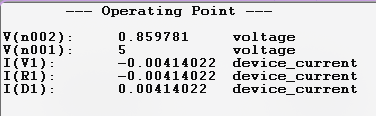
\includegraphics[width=0.7\linewidth]{figs/diode_op.png}
    \end{figure}
    \newline
$I_s$ of the diode chosen is $0.0154 fA$
\begin{enumerate}
    \item $r_d$ \begin{figure}[h!]
        \centering
        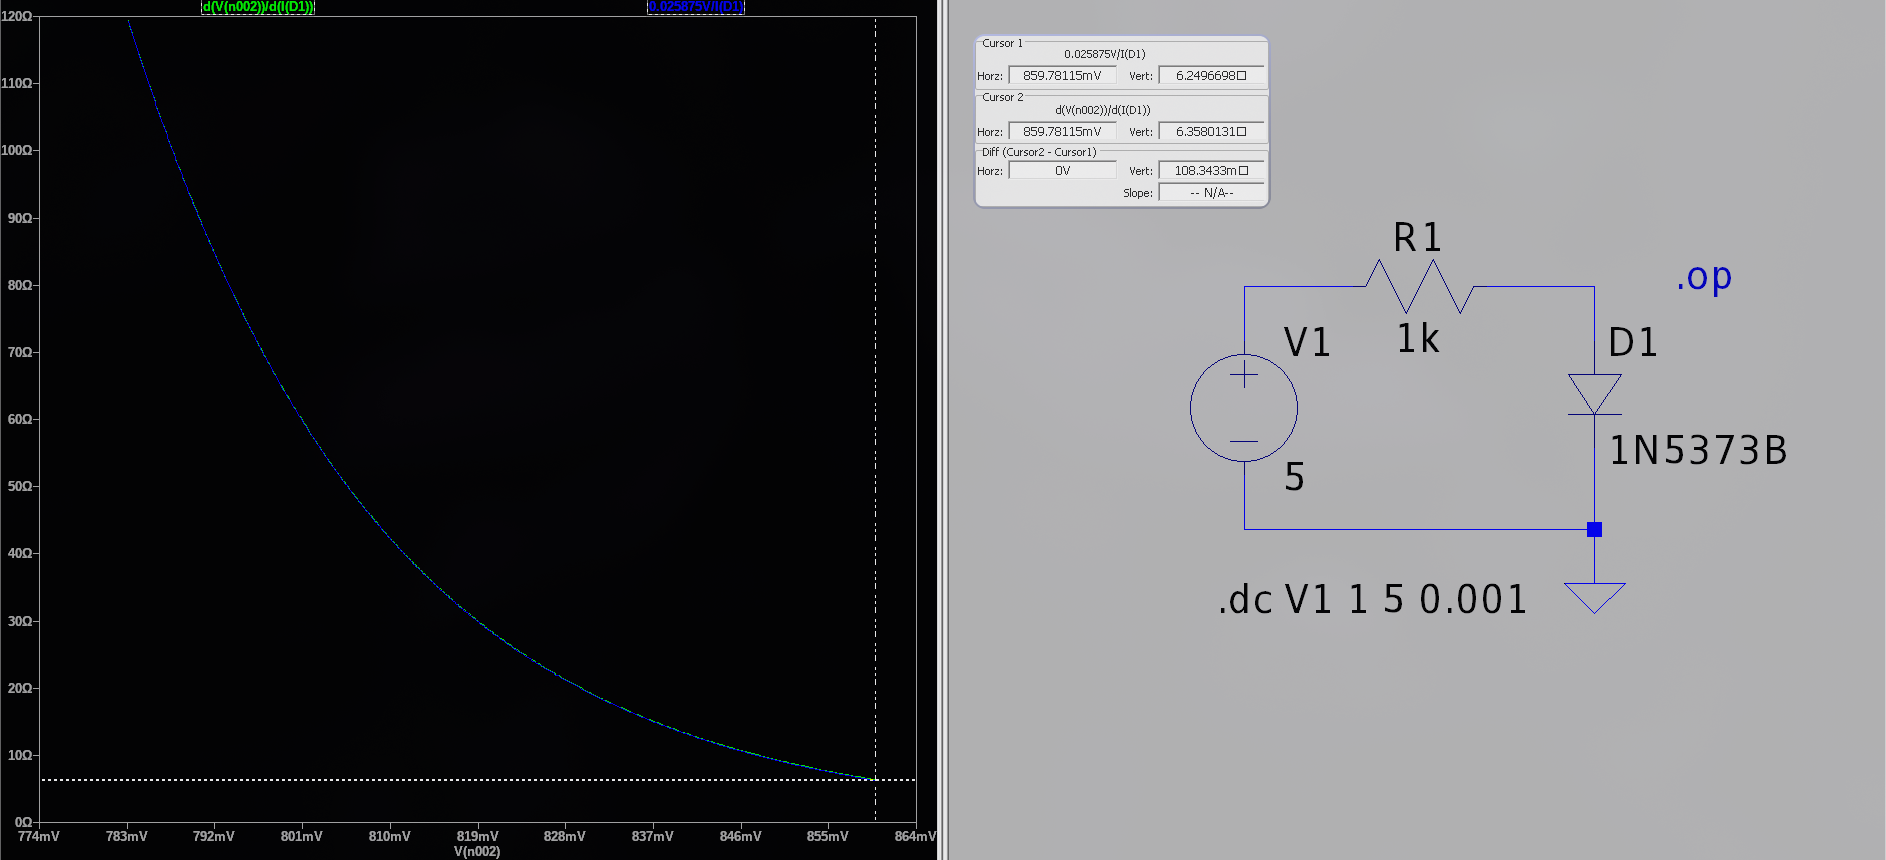
\includegraphics[width=0.9\linewidth]{figs/diode_rd.png}
    \end{figure}
    \item $I_s$ \begin{figure}[h!]
        \centering
        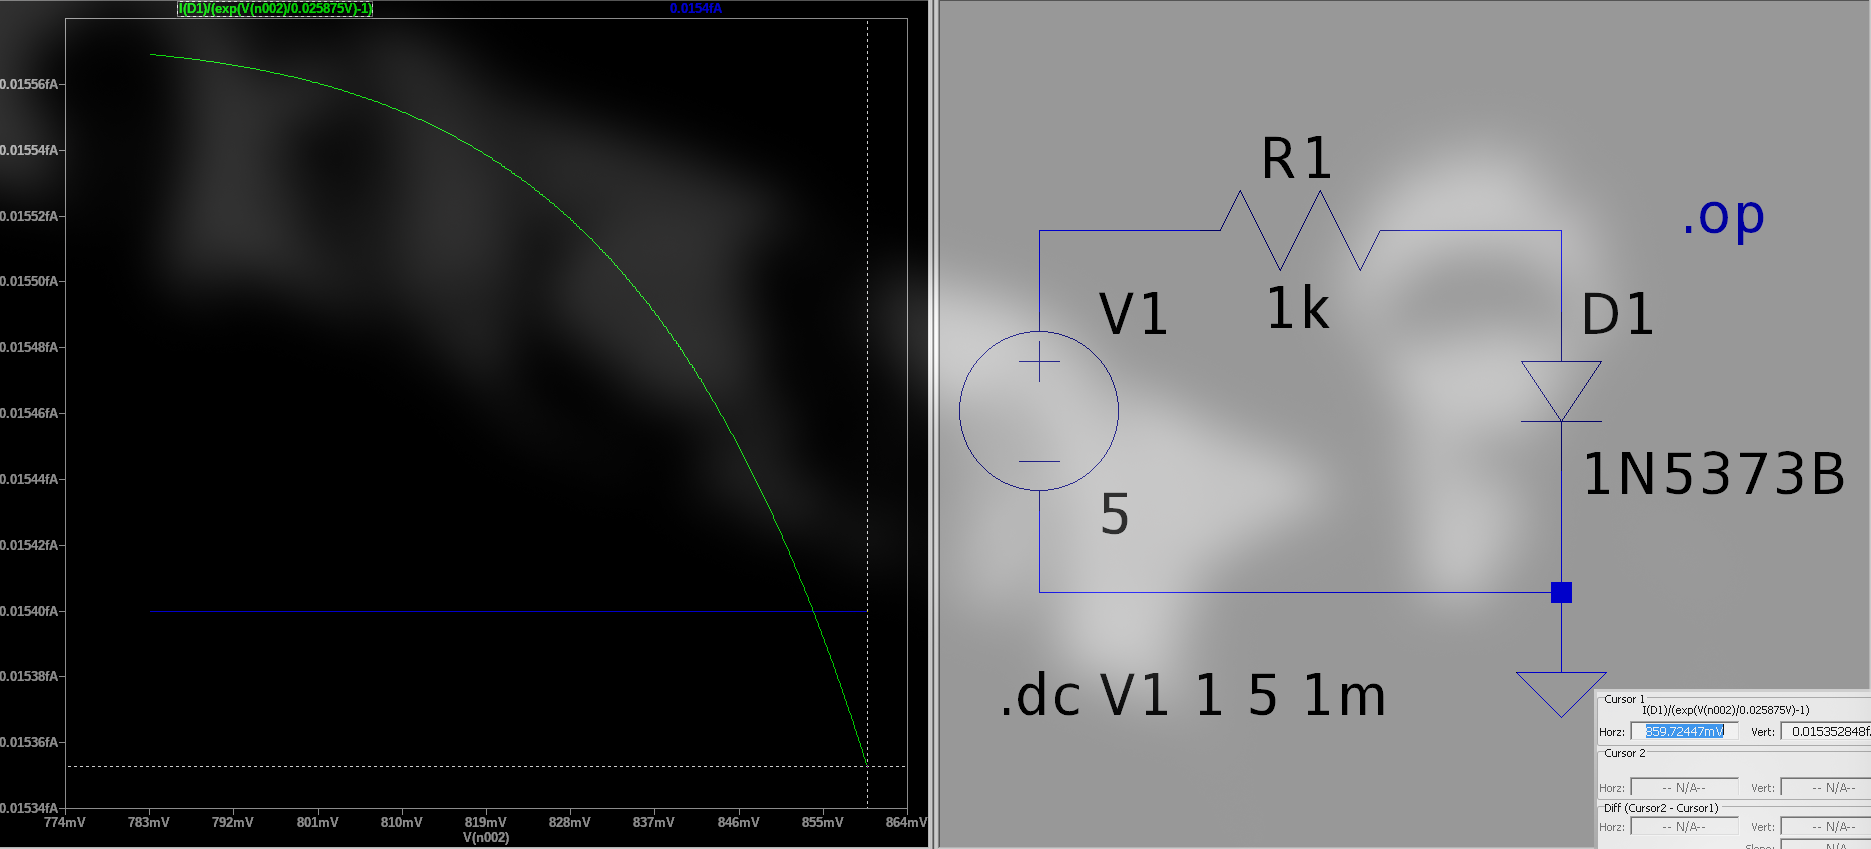
\includegraphics[width=0.9\linewidth]{figs/diode_is.png}
    \end{figure}
\end{enumerate}
\subsection*{Experimental vs Theoretical Results}
\begin{center}
\begin{tabular}{|c|c|c|c|}
\hline
Parameter & Experimental & Theory & Error (\%) \\
\hline
$r_d$ & 6.358 $k\Omega$ & 6.249 $k\Omega$  & 1.71 \\
$I_s$ & 0.01535 $fA$ & 0.0154 $fA$ & 2.27 \\
\hline
\end{tabular}
\end{center}
\pagebreak
\section{BJT}
\subsection*{Parameters and Formulae Used}

\begin{itemize}
    \item \textbf{Transconductance $g_m$}
    \begin{itemize}
        \item Hand Calculation: $g_m = \frac{I_C}{\eta V_T}$
        \item Experimental: $g_m = \frac{\partial I_C}{\partial V_{BE}}$ (from graph)
    \end{itemize}
    \item \textbf{Input Resistance $r_\pi$}
    \begin{itemize}
        \item Hand Calculation: $r_\pi = \frac{\eta V_T}{I_B}$
        \item Experimental: $r_\pi = \frac{\partial V_{BE}}{\partial I_B}$ (from graph)
    \end{itemize}

    \item \textbf{Current Gain $\beta$}
    \begin{itemize}
        \item Hand Calculation: $\beta = \frac{I_C}{I_B}$
        \item Experimental: $\beta = \frac{\partial{I_C}}{\partial{I_B}}$
    \end{itemize}

    \item \textbf{Output Resistance $r_o$}
    \begin{itemize}
        \item Hand Calculation: $r_o = \frac{1}{\lambda I_C}$
        \item Experimental: $r_o = \frac{\partial V_{CE}}{\partial I_C}$ (from graph)
    \end{itemize}
\end{itemize}
\subsection{Plots}
Operating Point values used,
\begin{figure}[h!]
        \centering
        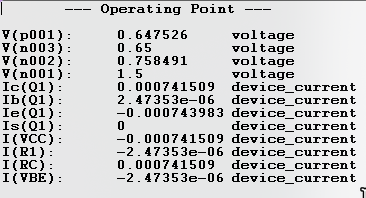
\includegraphics[width=0.7\linewidth]{figs/bjt_op_new.png}
    \end{figure}
For the BJT chosen, $\eta=1$
\pagebreak
\begin{enumerate}
    \item $g_m$ \begin{figure}[h!]
        \centering
        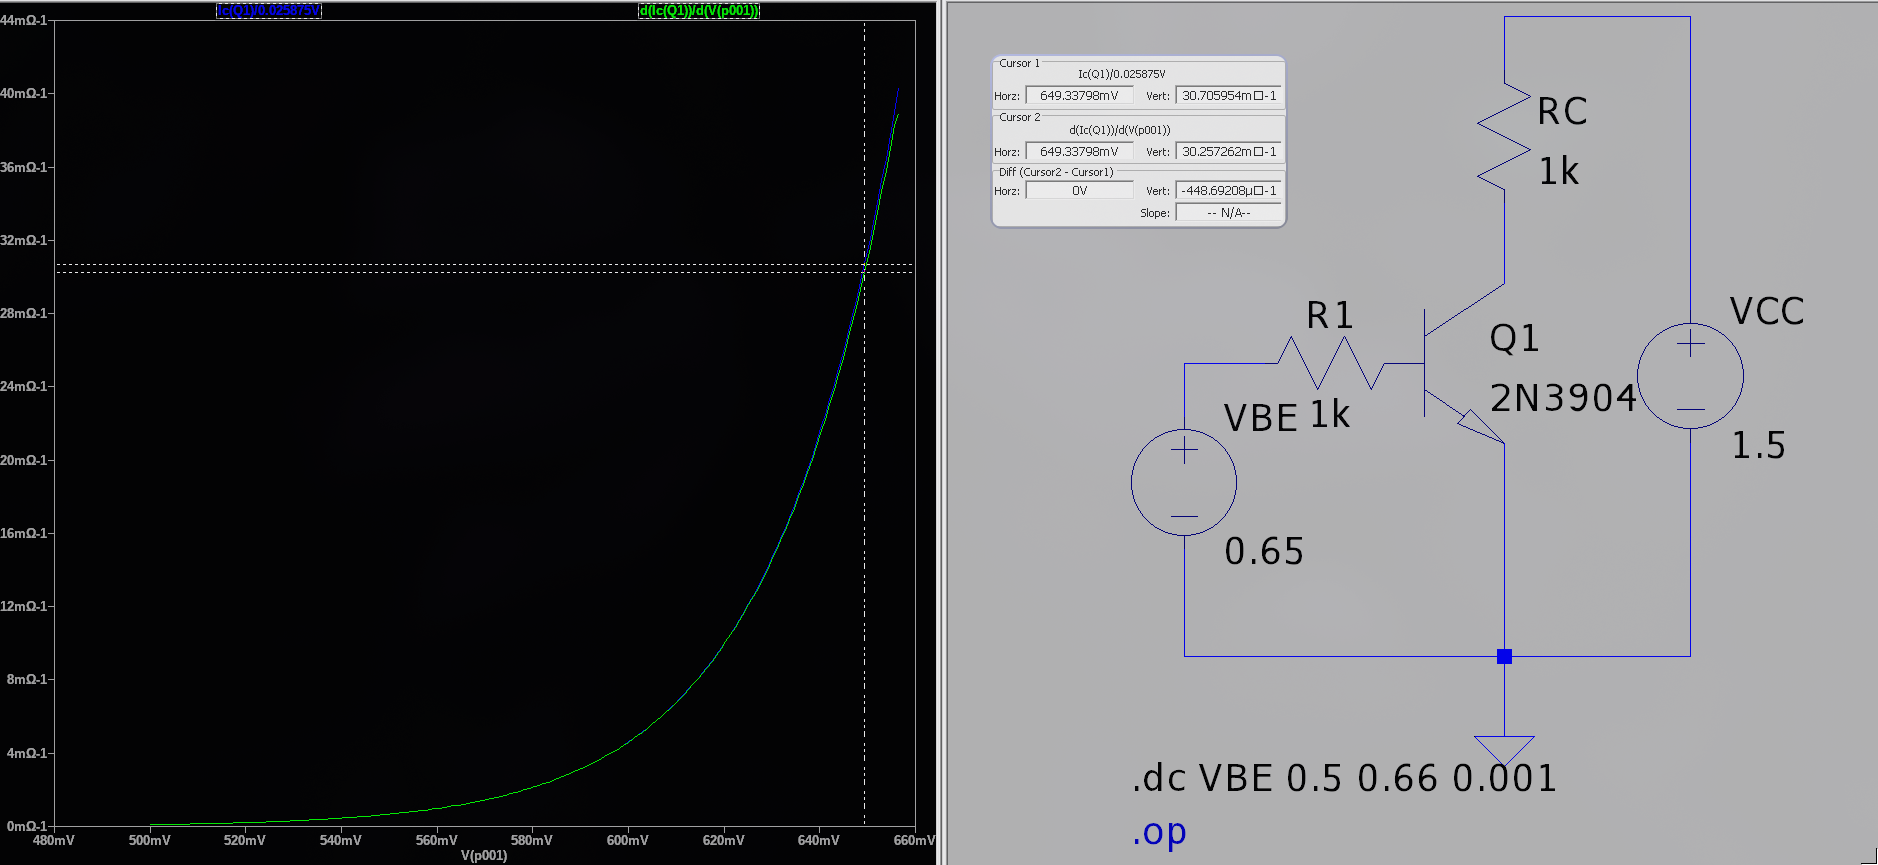
\includegraphics[width=0.9\linewidth]{figs/bjt_gm_new.png}
    \end{figure}
    \item $r_{\pi}$ \begin{figure}[h!]
        \centering
        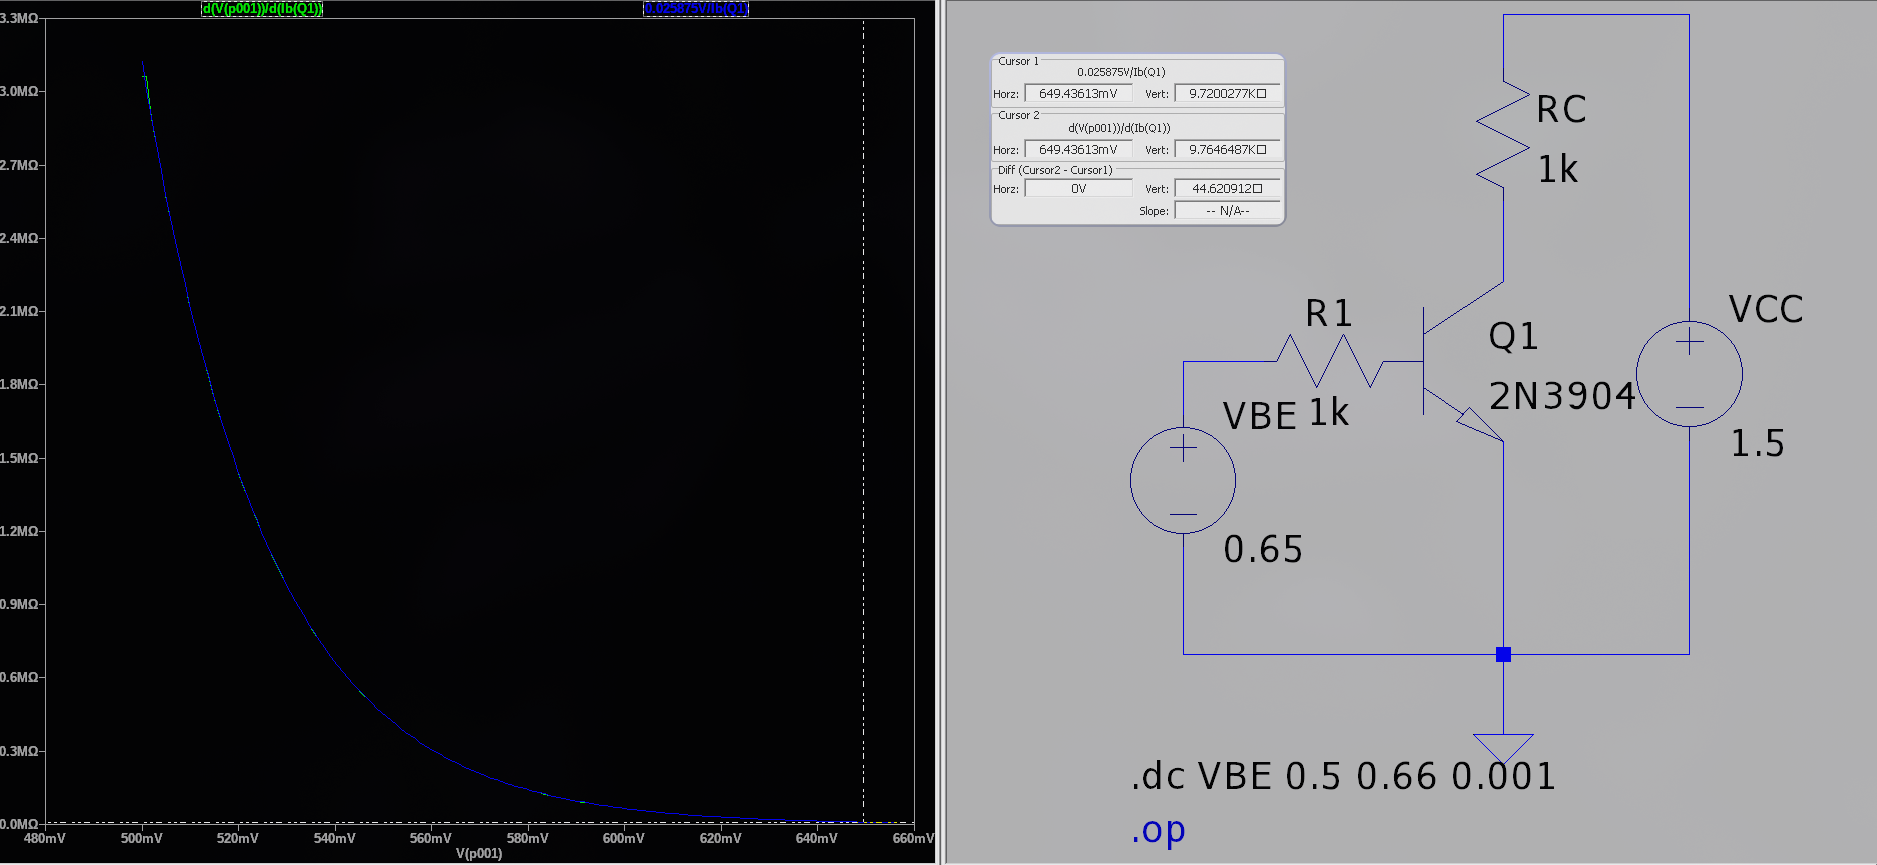
\includegraphics[width=0.9\linewidth]{figs/bjt_rpi_new.png}
    \end{figure}
    \item $\beta$ \begin{figure}[h!]
        \centering
        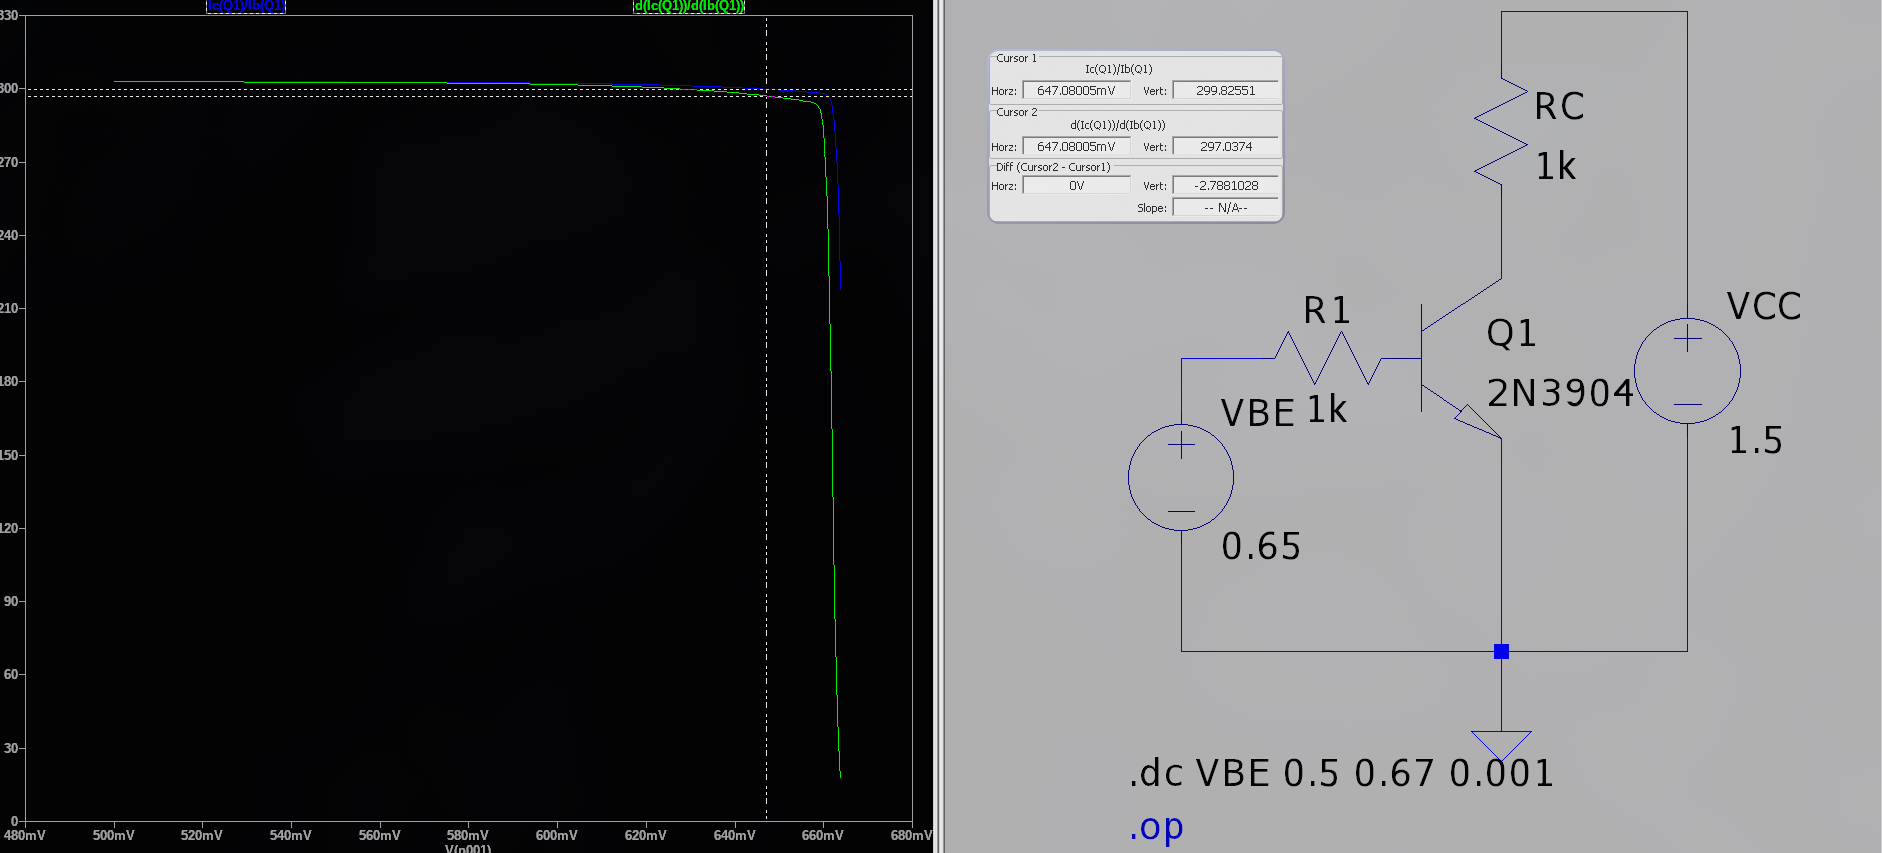
\includegraphics[width=0.9\linewidth]{figs/bjt_beta_new.png}
    \end{figure}
    \pagebreak
    \item $r_0$ \begin{figure}[h!]
        \centering
        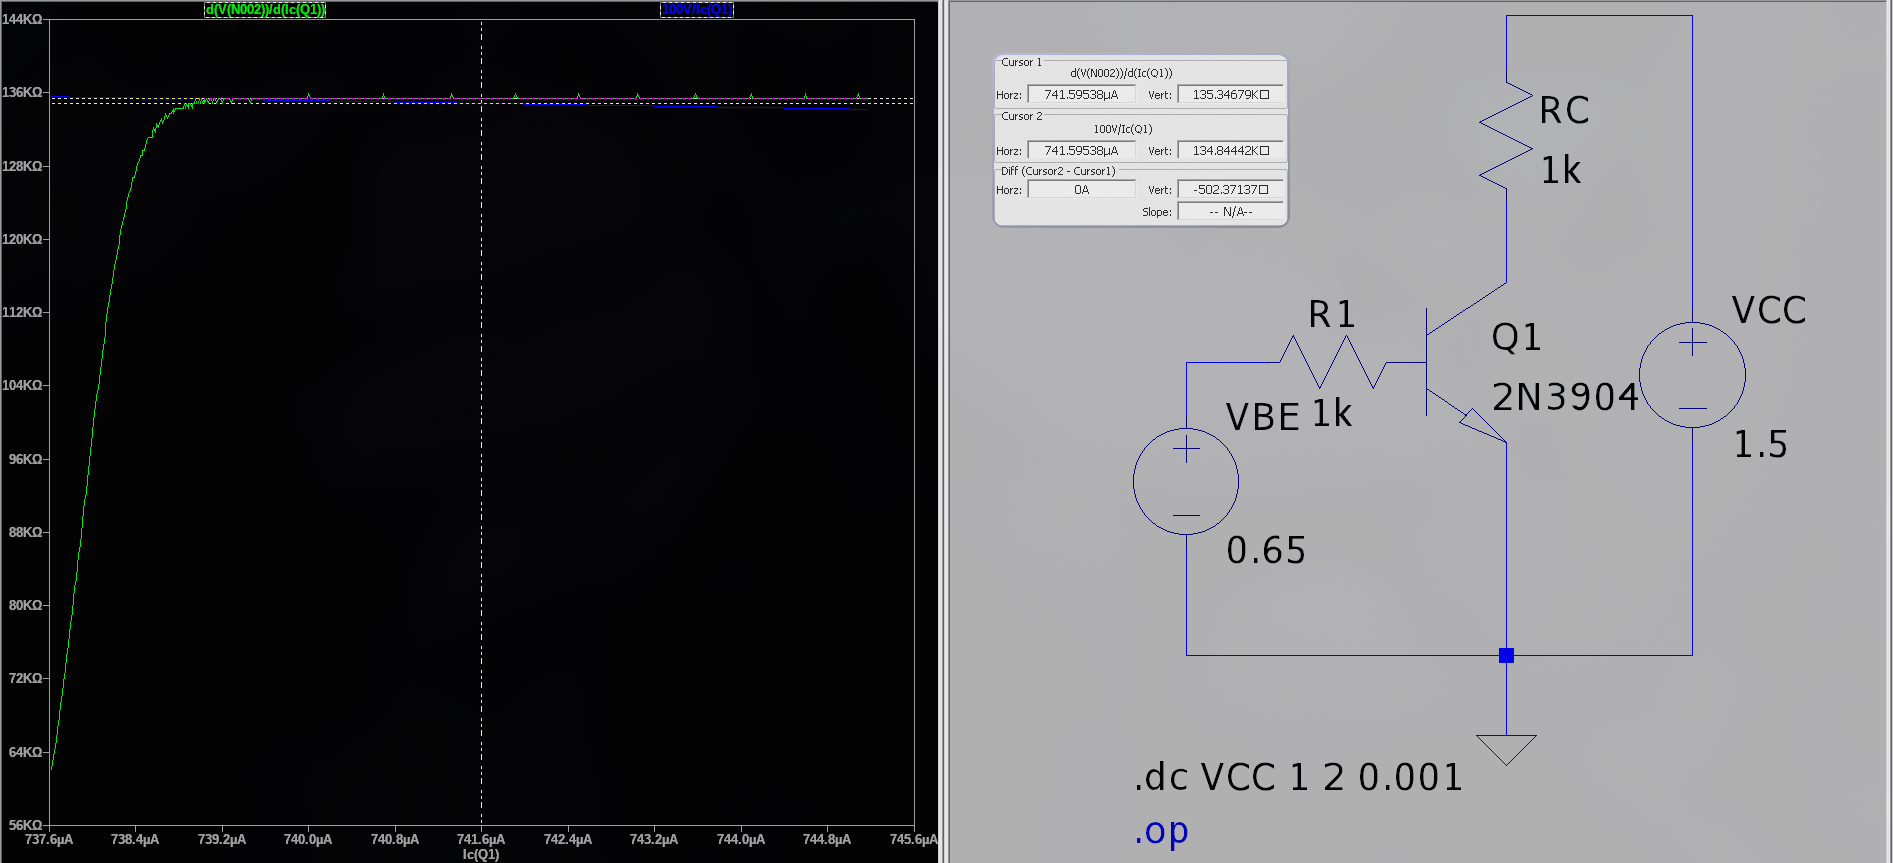
\includegraphics[width=0.9\linewidth]{figs/bjt_r0_new.png}
    \end{figure}
\end{enumerate}
\subsection*{Experimental vs Theoretical Results}
\begin{center}
\begin{tabular}{|c|c|c|c|}
\hline
Parameter & Experimental & Theory & Error (\%) \\
\hline
$g_m$    & 30.257  $m\Omega^-1$ & 30.705 $m\Omega^-1$ & 1.45 \\
$r_\pi$  & 9.764 $k\Omega$   & 9.720 $k\Omega$   & 0.45 \\
$\beta$  & 297.304 &   299.825                 & 0.93 \\
$r_0$ & 135.346 $k\Omega$ & 134.844 $k\Omega$  & 0.37 \\
\hline
\end{tabular}
\end{center}
\pagebreak
\section{MOSFET}
\subsection*{Parameters and Formulae Used}
\begin{itemize}
    \item \textbf{Transconductance $g_m$}
    \begin{itemize}
        \item Hand Calculation: $g_m = \frac{2I_D}{V_{GS}-V_{TH}}$
        \item Experimental: $g_m = \frac{\partial I_D}{\partial V_{GS}}$ (from graph)
    \end{itemize}
    \item \textbf{Output Resistance $r_o$}
    \begin{itemize}
        \item Hand Calculation: $r_o = \frac{\left( \frac{1}{\lambda} + V_{GS} \right)}{I_D} \approx \frac{1}{\lambda I_D}$
        \item Experimental: $r_o = \frac{\partial V_{DS}}{\partial I_D}$ (from graph)
    \end{itemize}
\end{itemize}
\subsection{Plots}
Operating Point values used,
\begin{figure}[h!]
        \centering
        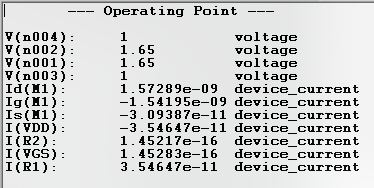
\includegraphics[width=0.7\linewidth]{figs/mosfet_op.png}
    \end{figure}
For the chosen MOSFET, $\lambda = \frac{1}{V_A} = 1000, V_{TH} = 0.025V$
\begin{enumerate}
    \item $g_m$ \begin{figure}[h!]
        \centering
        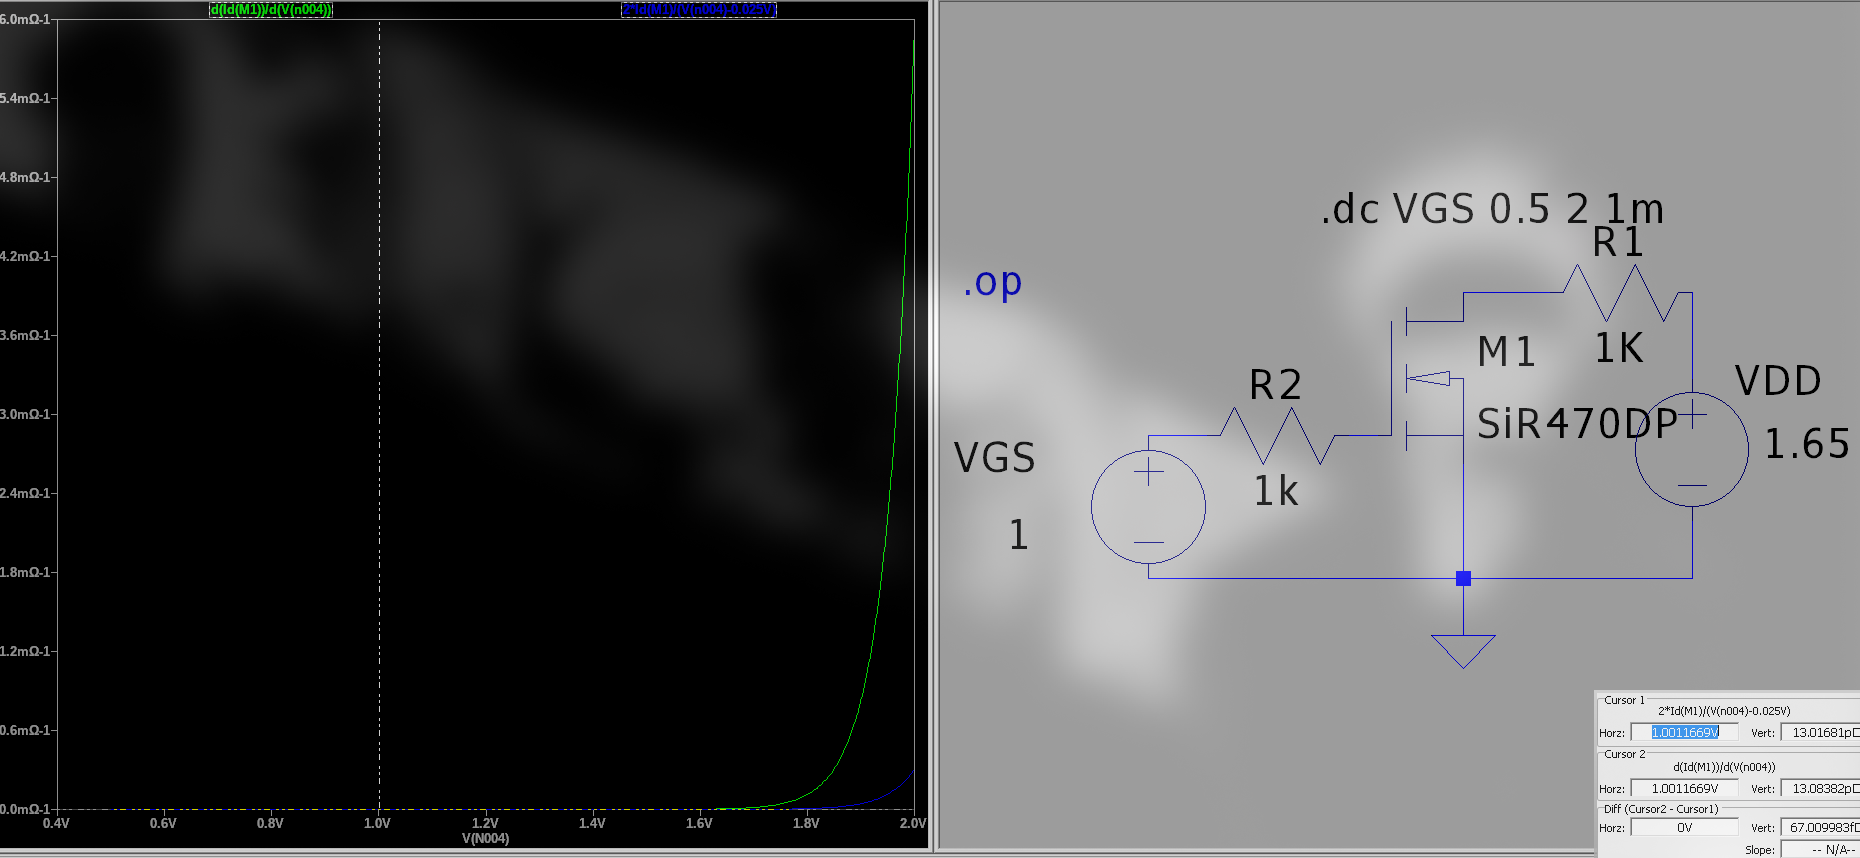
\includegraphics[width=0.9\linewidth]{figs/mosfet_gm.png}
    \end{figure}
    \pagebreak
    \item $r_0$ \begin{figure}[h!]
        \centering
        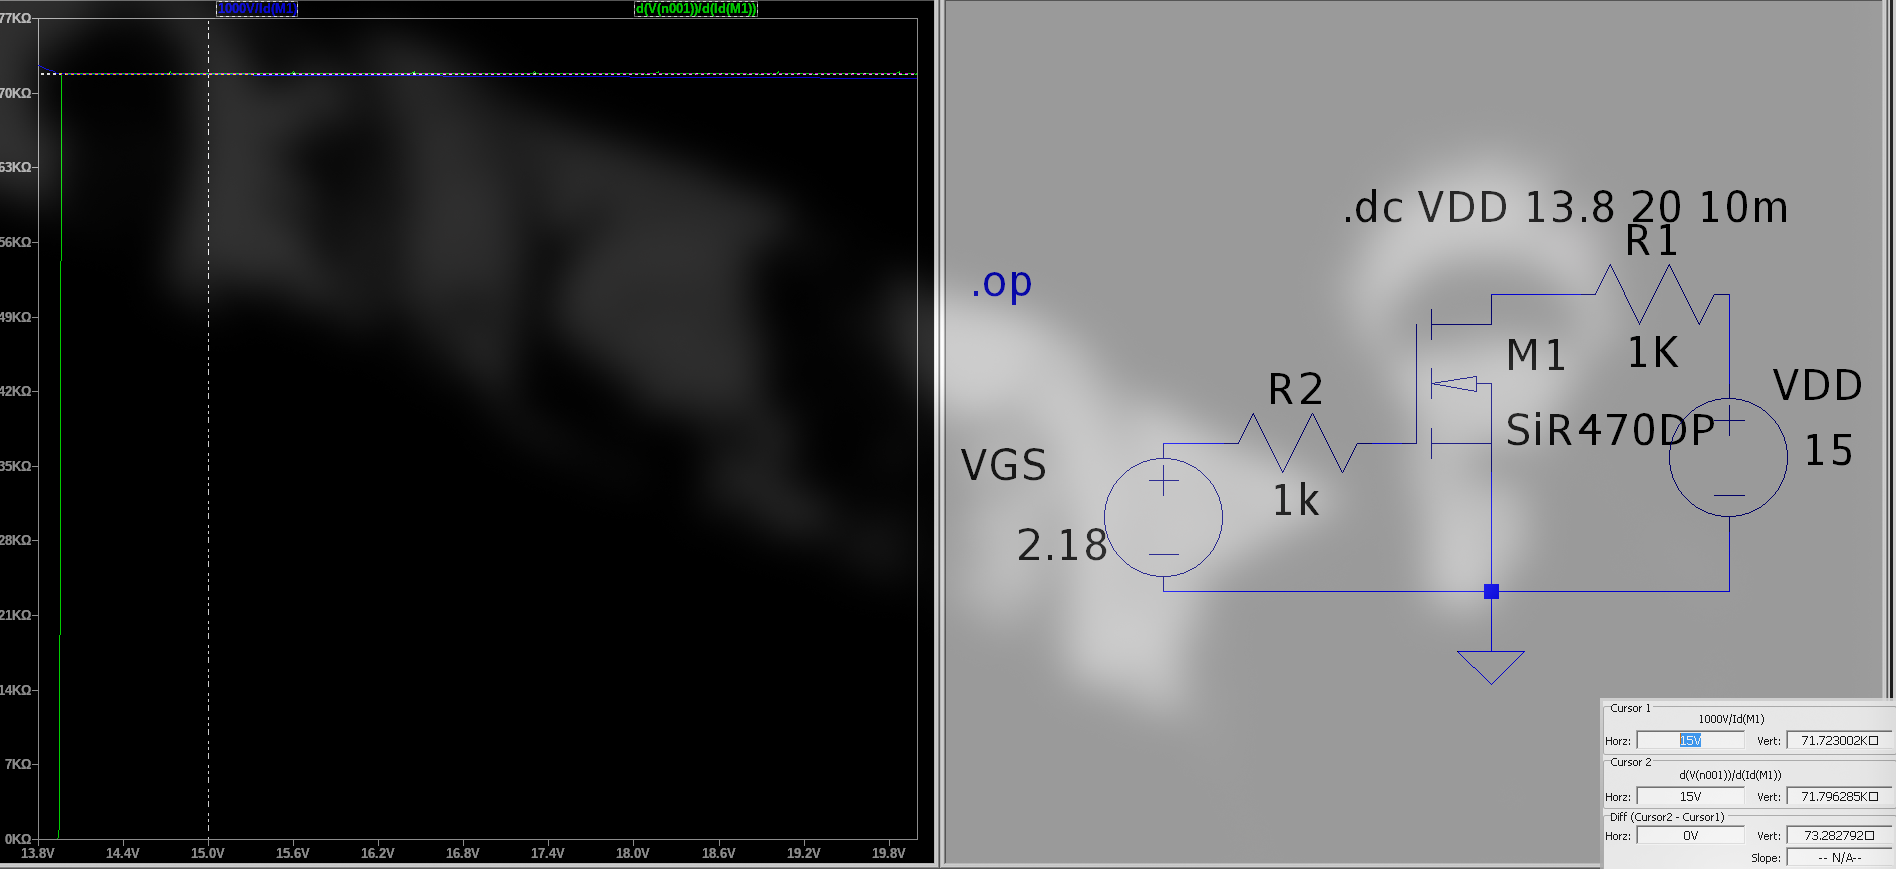
\includegraphics[width=0.9\linewidth]{figs/mosfet_r0_new.png}
    \end{figure}
\end{enumerate}
\subsection*{Experimental vs Theoretical Results}
\begin{center}
\begin{tabular}{|c|c|c|c|}
\hline
Parameter & Experimental & Theory & Error (\%) \\
\hline
$g_m$    & 13.083  $p\Omega^-1$ & 13.016 $p\Omega^-1$ & 0.51 \\
$r_0$ & 71.796 $k\Omega$ &  $71.723 k\Omega$  & 0.1 \\
\hline
\end{tabular}
\end{center}
\section{Conclusion}
The experiment to conduct small signal analysis and verify the parameters with hand calculations was successful with a maximum error of $5 \%$.
\end{document}